%=============================PREAMBLE=======================

% !TEX TS?program = pdflatexmk
		\documentclass[a4paper, 12pt]{article}
		\usepackage[english]{babel}
		\usepackage[utf8]{inputenc}
		\usepackage[utf8]{inputenc}		
		\usepackage{blindtext} 
		                    
%MARGINS
		\usepackage[left=25.4mm, right = 25.4mm, top=25.4mm, bottom=25.4mm, includefoot]{geometry}
		%\geometry{a4paper, total={170mm,257mm}, left=25.4mm, right = 25.4mm, top=25.4mm, bottom=25.4mm}
		\setlength{\parindent}{0in}
		\setlength{\parskip}{1em}

		
%CUSTOM LINE SPACING
		\usepackage{setspace}
		\setstretch{1.2}
		% \renewcommand{\baselinestretch}{1.0} 

                     
%HEADERS AND FOOTERS
		\usepackage{fancyhdr}
		\pagestyle{fancy}
		% \fancyhead{}
		\fancyfoot{}
		\fancyfoot[R]{ \thepage\ }
		 \renewcommand{\headrulewidth}{0pt} %change the pt width to insert header line
		\renewcommand{\footrulewidth}{0pt} %change the pt width to insert footer line
		\usepackage{amsmath}
		\fancyhf{}
		\rfoot{Centre for Civil Society \hspace{1mm} \textbar \hspace{1mm} www.ccs.in \hspace{2mm}  \thepage}
                    
		% \rhead{\leftmark}
		% \lhead{Guides and tutorials}
		% \lfoot{  \leftmark }     			% get the section heading on the footer 
		
                                    
%TABLES
                    \usepackage{booktabs}
                    \usepackage{subfig}
                    \captionsetup{aboveskip=14pt,}
                    \captionsetup[table]{singlelinecheck = false}
                    \usepackage{array}
                    \usepackage{makecell}	
                    \usepackage{multirow}
                    \usepackage{multicol}
                    
                    
%COLORED BOXES
                    \usepackage{xcolor}
                    \usepackage{mdframed}


%LISTS                    
		\usepackage[shortlabels]{enumitem}
       
                    
 %DEFINING COLOURS
		\definecolor{CCSbrown}{RGB}{163, 86, 37}
		\definecolor{CCSgrey}{RGB}{105, 105, 105}
                 \definecolor{CCSblack}{RGB}{64, 64, 65}     
                 
                                  
%HEADING COLORS            
		\usepackage{sectsty}
		\usepackage{titlesec}
    		\chapterfont{\color{blue}}  % sets colour of chapters font
    		\sectionfont{\color{CCSbrown}}  %sets colour of section font
    		\subsectionfont{\color{CCSblack}} %sets colour of subsection font
    		\subsubsectionfont{\color{CCSblack}} %sets colour of subsubsection font
    			
%ADDING PICTURES
		\usepackage{graphicx}
		\usepackage{float}
              
%BIBLIOGRAPHY and LINKS
		\usepackage[authordate, backend=biber]{biblatex-chicago}
		\addbibresource{ewaste_v2.bib} %need to change to restaurants bib           
 		\usepackage{hyperref} 
		\hypersetup{
			colorlinks,
			linkcolor = black,
			citecolor = blue}               
  
\begin{document}
                    
    %==================================================                
                    %TITLE PAGE
                    
                    \begin{titlepage}
                    \begin{center}
                    	
			\line(1,0){300}\\
                    	[0.25in]
                    	\huge{\bfseries \textcolor{CCSbrown} {A Seven Course Dilemma}} \\
    			[0.5cm]
    			\large  {Examining the Ease of Doing Business for Restaurants in Delhi} \\%modified title from proofed version. i think each paper should have a strong verb beginning in the byline
    	
                    	\line(1,0){200}\\
                    	[4in]
                    	\LARGE {Parth Gupta, Rutvi Vadera, and Retika Vijay} \\ % ewaste has some off norm about line space after first author. can you please check and confirm convention; also i am removing small caps. this way it fit on one line. also added 'and'
                    	[2cm]
                    	{\Large Centre for Civil Society} \\
                    	{\normalsize New Delhi, India} \\
			{\normalsize September 2018} \\
    			
			%[2.0cm]
    			% 
\includegraphics[width = 75mm]{CCSlogo.jpg} - needed the logo so haven't inserted
      
                    \end{center}
                    \end{titlepage}
                    
                 
  %=====================TOC===============================================                 
                    \tableofcontents
                    
                    
 %======================LIST OF ABBREVIATIONS================================         
                   \newpage
                   \newlist{abbrv}{itemize}{1}
                   \setlist[abbrv,1]{label=,labelwidth=1in,align=parleft,itemsep=0.1\baselineskip,leftmargin=!}
                   
                   \section*{List of Abbreviations}
                   \addcontentsline{toc}{section}{List of Abbreviations}
                  
        
        \begin{abbrv}        
        
 		\item[CTE]		Consent to Establish
 		\item[CTO]		Consent to Operate
 		\item[DFS]		Delhi Fire Services
 		\item[DoT]			Department of Tourism
 		\item[DPCC]		Delhi Pollution Control Committee
 		\item[FBO]		Food Business Operator
 		\item[FSC]		Fire Safety Certificate
		\item[FSSAI]		Food Safety and Standards Authority of India 
 		\item[FSSR]		Food Safety and Standards Regulations
 		\item[GST]		Goods and Services Tax
 		\item[HTL]			Health Trade Licence
 		\item[MCD]		Municipal Corporation of Delhi
 		\item[NBC]		National Building Code
 		\item[NDMC]		New Delhi Municipal Corporation
 		\item[NOC	]		No Objection Certificate
 		\item[NRAI]		National Restaurant Association of India  
               \end{abbrv}

%should we be checking the list again for comprehensiveness? i suspect there are more abbrvs that are not listed here. for all papers. 

        
   %=============TODO and NOTES
   		% have not integrated refs to the doc yet. refs are still in brackets
		% need to check for bold/italics/underline
		% hyperrefs were working in the morning, now are not
		% need to add tables/clean tables
		% do we need to hyperref tables/figures where referenced?
		% unable to do enumerate A,B,C
		% i would like to change the styling of the title page: the title of the paper should be the most prominent, authors not in caps, authors/date/ccs should go slightly more to the bottom half of the page
		% also should we do superscript for 'th' and how?
		% need to check off alston's list
		% figures are untidy. will help to rework the source files
		% need to change para spacing in the appendix. ugly spacing. not able to figure out how to customize. 
		% the title page needs to be different only when we are putting the papers as individual docs on the website. for fnf/atlas report, we don't need ccs+date on each chapter title?
		% restyled the title page. if this works, we can redo all papers like this.   
		
         
 
   %======================EXECUTIVE SUMMARY================================  
                        
                    \newpage
                    \section*{Executive Summary}
                    
                    \addcontentsline{toc}{section}{Executive Summary}
                    
                    The Indian Food Services market, comprising restaurants, cafes, bars and street kiosks stalls, is estimated to reach Rs. 498 thousand crores and contribute 2.1\% to the Gross Domestic Product of the country by 2021 (Maheshwari et al. 2016, p. 4). 
Despite the growth outlook, 66\% of the industry remains unorganised (ibid, p. 3).\footnote{Unorganised eating houses do not conform with the following parameters: (i) accounting transparency; (ii) organised operations with quality control and sourcing norms; and 
(iii) outlet penetration (Dabas 2017, p. 9).}  We study the legal and regulatory framework in Delhi that governs the food services business and captures the experience of owners and managers operating under the framework.
                   
          Any eating house in Delhi faces cumbersome and often overlapping regulations. An alcohol-serving restaurant needs to acquire 11 licences (or 13 if they play recorded music and choose to install a lift) and submit 57 documents before they open shop legally 
(Appendix 1). The process is daunting in the absence of procedural clarity, dysfunctional communication channels between the government and enterprises and technical difficulties.  
                    
                    Through a structured survey of restaurant owners, interviews with government officials and an analysis of secondary information, we find that it takes 120 to 150 days to obtain all licences, if there is no delay beyond the officially stipulated time, and the 
formal cost varies from Rs. 18,300 to Rs. 1,852,087 (Tables 1 and 2).\footnote{Excluding the cost of the Signage Licence, which is calculated based on the surface area of advertising boards.} More than half of all respondents in our survey found the overall 
licensing procedure to be difficult or very difficult to follow. An Excise Licence, rated the most arduous of all by the respondents, costs restaurants anything between Rs. 7.64 lakhs and Rs. 18.52 lakhs annually. 
                    
                    Even if restaurateurs manage to fulfil all the licensing requirements to open, they are plagued by an extortionary inspections regime and arbitrary changes in rules. An inspection system ought to maximise compliance by providing relevant information to 
enterprises, including easily accessible guidance material, checklists and toolkits. Out of the 12 departments that regulate the operations of a restaurant in Delhi, only one has published a guidance document, leaving restaurateurs without any information about the 
inspection procedure followed by other departments. In fact, a major complaint of the interviewed restaurateurs was the lack of a single point to access clear guidelines to be followed while operating a restaurant.
                    
                    Besides this, restaurants face frequent and arbitrary government orders that directly impact the operations of a restaurant, often adversely. For example, in May 2018, the Department of Excise in Delhi banned liquor-serving restaurants from playing 
recorded music on the grounds of ‘nuisance caused by high volumes’.\footnote{\href{https://bit.ly/2MzCM02}{Order No. 2(72)/Ex/Restt/Misc./2016-17/1567 (2018)} from the Office of Excise Commissioner, Delhi (dated 9 May 2018).} In another instance, the New 
Delhi Municipal Corporation (NDMC) banned the use of rooftops by restaurants and bars following a mishap in Connaught Place in December 2017 (The Times of India 2017). A restaurateur at Hauz Khas estimated a 60\% loss in business  within 2 days of the ban, 
as his was one of the few restaurants providing rooftop dining—the primary attraction for his customers (Kaushik 2015). % edited the last sentence after the proofing version for incorrect grammar. 
                    
                    Devising reactionary rules without a robust debate does not make us safer or better protected. Such changes undermine confidence in any market, increase short-term costs for businesses and create distrust in government actions. To encourage 
growth in the sector, it is imperative to declutter the current regulatory framework while protecting customers and the general public from health hazards and nuisance. 
                    
                   The paper explores the current regulatory framework with the intention to initiate a discussion on the regulatory hygiene required for food service enterprises to thrive. The paper is organised as follows: the \hyperref[intro]{introduction} sets the context of 
the research. This is \hyperref[sec:1]{followed} by an enumeration of all the licences required to open a restaurant, and the official cost and the stipulated time taken to obtain them. Here we also present the experience of restaurateurs in obtaining these licences 
and the procedural ambiguities in obtaining each licence. \hyperref[sec:2]{Next}, we discuss the perception of restaurateurs on the inspections regime. \hyperref[sec:3]{Finally}, we highlight the pressing pain points that business owners encounter while running a 
restaurant, followed by a \hyperref[end]{conclusion}.  %added a comma in sentence3.  minor edit in 4th sentence from proofed version. also 'finally'. 

    %======================INTRODUCTION================================                     
                    \newpage
                    \section{Introduction}
                    \label{intro}
                    Public interest theory of regulation postulates that regulation reduces market failures and ensures that those who enter the market bring in a high quality of goods and services (Hertog 2010, p. 3). Registration gives new companies a type of official 
approval that they are reputable enough to engage in transactions with the general public and other businesses (SRI 1999, p. 14). Contrastingly, public choice theory argues that in practice, regulations work in favour of existing firms by limiting the entry of new firms 
and ‘give officials the power to deny them and to collect bribes in return for providing the permits’ (Stigler 1971, p. 3)(Shleifer and Vishny 1993, p. 601). %we have a reference problem. stigler was not a public choice theorist though he did add to the school of thought. 
                    
                    Other researchers (Bardhan 1997, p. 1322) have argued that ways to circumvent regulations, such as payment of bribes, can sometimes be effective, in principle, if it aids the release of entrepreneurs from regulation, or reduces the delay in issuing of 
licences. However this works out, the additional burden imposed on businesses is distortionary (Djankov 2002, p. 3) or subjects the entrepreneur to ‘some of the worst treatment imaginable... and presenting the investor with insurmountable delays or repeated 
obstacles unless he makes a large payoff’ (Emery 2000, p. 10). 
                    
                    These arguments partially explain why more than two-thirds of the Rs. 309100 crore food services industry that employs an estimated 5.8 million people (Maheshwari et al. 2016, p. 4) remains unlicensed (ibid, p. 5). Kaushik (2013, p. 30) studies the 
regulatory framework for formal and informal eating houses and describes the process of registration ‘as a maze where an entrepreneur can easily lose his way’. 
                    
                    To improve the ease of doing business, the central and state governments have introduced legislative and regulatory changes, such as the introduction of the Goods and Services Tax (GST). However, when it comes to reforms, there is an insufficient 
focus on the services sector and especially on what ‘remains one of the biggest challenges’ for the food services sector, that is, starting an enterprise (ibid, p. 18). High barriers to entry leave entrepreneurs in the food service industry with three choices: change their 
occupation; succumb to the extra-legal space and operate informally; or give in to the demands for ‘facilitation payments’.
                    
                    As our main contribution to the research on the ease of doing business in Delhi, we have described the existing licensing regime for eating houses in the state. We provide a list of all licences required to set up a restaurant in Delhi supplemented with 
the perception of the restaurateurs of the ease of obtaining each licence. Through the responses of restaurant owners and managers, we have also highlighted the challenges they face such as document requirements, information accessibility, uncertain regulatory 
environment and procedural timelines.
                    
                    The findings are based on a survey of 101 food services enterprises in South Delhi (See \hyperref[Appendix 2]{Appendix 2}). Respondents include owners, managers and sometimes chefs of full-service restaurants, quick service restaurants and cafe 
and bars.\footnote{Street kiosks stalls were not included in the survey.} Our interest in Delhi was due to two reasons: first, it is one of the two cities studied by the World Bank to create rankings for the Ease of Doing Business in India; and second, Delhi is one of the 
tourist hotspots of India, ranked 4th in India for attracting foreign tourists and 15th for attracting domestic tourists, as of 2016 (India Tourism Statistics 2017).
                    
                    The paper is organised into four sections: licences required to start a restaurant in Delhi, the perception of restaurateurs of the multi-agency inspections regime, the challenges that the restaurateurs face in running their business and a conclusion. 
% re-edited intro. it was not flowing nicely and paras were currently too small. 
            
                                        
%======================Regulatory Framework for Restaurants in Delhi======================
                    \section{Regulatory Framework for Restaurants in Delhi}
                    \label{sec:1}
                    In this section, we describe the procedure for obtaining mandatory and service-specific licences, as well as the time and cost of following these procedures for eating houses in Delhi. We list the licences that need to be acquired before a restaurant can 
officially open its doors, the official cost of obtaining these licences and the minimum time it takes to meet them, assuming no delays. Wherever necessary, we highlight the ambiguities and contradictions that exist in the licensing procedure. We also document the 
experience of restaurants based on a survey asking enterprises to rate their experience of obtaining each licence from options ranging from very difficult to very easy.
                    
                    
                    \subsection{Mandatory Licences: Enumerated Process and Procedural Ambiguities}
                     Any entrepreneur looking to set up an eating house in Delhi requires a minimum of eight licences enlisted in Table 1.\footnote{According to Delhi Police Act 1978 (Chapter 1), ‘eating house’ means any place to which the public are admitted and where 
any kind of food or drink is supplied for consumption on the premises by any person owning, or having any interest in or managing such place and includes a refreshment room, boarding, coffee house, a shop where any kind of food or drink is supplied for 
consumption in or near such shop but does not include a place of public entertainment.} The officially stipulated fee ranges from Rs. 18,300 to Rs. 38,500, depending on the revenue and seating capacity.\footnote{Excluding the cost of a Signage Licence, which is 
calculated based on the surface area of advertising boards.} In the absence of a single-window clearance system, the process of acquiring licences takes around 120 to 150 days (Maheshwari et al. 2016, p. 23). All except one of these processes can be conducted 
online.
     
                   In contrast, it takes four licences in China and two in Turkey (Philip 2015). In Hong Kong (‘"Starting A Restaurant in Hong Kong’ 2018), the Food Business Operator (FBO) only has to acquire the General Restaurant Licence issued by the Hong Kong 
Food and Environmental Hygiene Department before commencing operations.

%Table 1: Time, Cost, Validity and Procedure of Mandatory Licences in Delhi
 %table 1 needs to go here. also table 1 has footnotes #7/8/9 from the word doc. 
                    
                                        
                    \subsubsection{Food Licence}
                    A food licence, issued by the Food Safety and Standards Authority of India (FSSAI), is mandatory for any food-related business and is the primary requirement to set up a restaurant in Delhi. Depending on the turnover, over a third of our survey 
respondents termed the process of obtaining this licence as ‘difficult’ or ‘very difficult’ to navigate through (Figure 1). The food licence can be obtained only online through the department website.
                    
                    An eating house can apply for three types of FSSAI Licences: Central Licence, State Licence and Registration Certificate. The licences are issued at two levels of the government. The Central Licence is issued by the FSSAI department at the Centre. 
The State Licence and Registration Certificate are issued by the Department of Food Safety under the Government of Delhi.
                    
                    The type of licence an eating house must obtain depends on whether it plans to operate in more than one state and their turnover. However, discrepancies exist in the application criteria specified in the Food Safety and Standards Regulations 
(FSSR) 2011 and the website of FSSAI. The FSSR 2011 requires that FBOs ‘operating in two or more states’ obtain a Central FSSAI Licence, whereas the website of FSSAI website states that FBOs with turnover more than 20 crores are required to obtain a 
Central FSSAI Licence.\footnote{According to the FSSR 2011, Schedule I, Point 9, FBOs operating in two or more states have to apply for a Central FSSAI Licence.} \footnote{\href{https://bit.ly/2pbFEXM}{Central FSSAI Eligibility Criteria} (Accessed 31 June 
2018)}.
                    
                    It is unclear what a restaurant with a proposed turnover of over Rs. 20 crores but operating only in one state should do. %this para was highlighted in the paper. i don't know how to do this, or if we should. 
                    
% Table 2: Conflicting Information Provided by the FSSR 2011 and the Website of FSSAI
		\begin {table}
		\raggedright
		\caption{Conflicting Information Provided by the FSSR 2011 and the Website of FSSAI\footnote{Food Safety and Standards Regulations, 2011, Schedule I, Point 9.}}
		\begin{tabular}{l | l | c | c}
			\multirow {2}{*}{\bf{\thead{Turnover}}} & \multirow {2}{*}{\bf{\thead{Information Source}}} & \multicolumn {2}{c}{\bf{\thead{Type of License}}}\\
			& & \textit{\footnotesize{Single-state Operations}}	&	\textit{\footnotesize{Multi-state Operations}}\\
			\hline
			\hline
			\multirow {2}{*}{$<$ Rs. 20 crores}	&	FSSR 2011		&	State Licence	&	Central Licence\\
			&Website of FSSAI	&	State Licence	&	Central Licence\\
			\hline
			\multirow {2}{*}{$>$ Rs. 20 crores}	&	FSSR 2011		&	\textcolor{red}{State Licence}	&	Central Licence\\
			&Website of FSSAI	&	\textcolor{red}{Central Licence}	&	Central Licence\\
			\hline
		\end{tabular}
		\end{table}  		

%having some trouble with footnote in the caption = footnote text isnt showing up; also need to make the table prettier



%table 2 needs to go here. table 2 has footnote 12, and hyperlink to FSSAI site. also can we not say 'fssai's website instead of website of fssai?   
                    
                                    
                    \subsubsection{Health Trade Licence}
                    Among the 13 licences we sought feedback on, the Health Trade Licence (HTL) was the second most difficult to obtain. Fifty-one out of 93 (55\%) respondents termed it as either ‘difficult’ or ‘very difficult’ to obtain (Figure 1). The Municipal Corporation 
of Delhi (MCD) issues an HTL under Section 421 of The Delhi Municipal Corporation Act, 1957, to validate the safety and hygiene of a restaurant.
                    
                    The HTL is seen as difficult to obtain due to several reasons. For instance, a manager of a cafe lamented that even if the process of obtaining the licence was online, he had to visit the office to get the verification done faster. Another restaurateur said 
that his application was stalled deliberately on various occasions on the pretext of ‘insufficient documents’ without any further clarification until he visited the office. Bribery was cited as a common practice. An interviewee stated, ‘bribery or commission payments is 
the traditional way of doing business. You can’t do a thing without paying up in this business’.
                    
                    According to the online application portal of Municipal Corporations, the validity of the HTL is 1 year.\footnote{\href{https://bit.ly/2Qzd92r}{Validity Chart of the HTL for SDMC} (Accessed 16 June 2018).} However, that is in conflict with what the Municipal Corporations claim: the validity is ‘one financial year’, that is the licence is valid up to 31 March of each year, irrespective of the date of issue/date of generation of licence. As per the Twelfth Schedule of The Delhi Municipal Corporation Act 1957, a fine of Rs. 100 can be levied in case of a non-renewal of the HTL. %this para was highlighted in the paper. i don't know how to do this, or if we should.     
  
     
		\subsubsection{Fire Safety Certificate}
		The restaurants we surveyed had a seating capacity ranging from 5 to over 100; however, 17 of 101 restaurants had a seating capacity of exactly 48. The criterion for eligibility for a Fire Safety Certificate (FSC) partially explains this clustering. The 
certificate, issued by the Delhi Fire Services (DFS) under the Delhi Fire Service Act 2007 (Delhi Act 2 of 2009) and the Delhi Fire Service Rules 2010, is required only if the number of seats in the restaurant is 50 or above. Since obtaining an FSC from the DFS 
necessitates the installation of fire safety equipment, many restaurants limited themselves to 48 seats. %what is (Delhi Act 2 of 2009)
		
		Not all eating houses have to apply to obtain an FSC. Only ‘Assembly buildings’ need to apply for an FSC. The DFS has revised the criteria based on the guidelines mandated by the National Building Code (NBC), 2005, for identifying an ‘Assembly 
building’. Earlier, all buildings with a seating capacity of 50 or more were categorised as ‘Assembly buildings’ (Delhi Fire Services Act, 2007). Now, a revised formula based on floor area is used to determine if the venue is an ‘Assembly building’ and will require an 
FSC.\footnote{Floor area/1.5 sq. metres.} 
		
		When a restaurateur applies for an HTL, it is the responsibility of the local municipal corporation to which they are applying to verify if the eating house falls under the category of ‘Assembly building’ and to direct the applicant to the DFS to apply for an 
FSC.\footnote{The NCT of Delhi is governed by three Municipal Corporations: NDMC, the Delhi Cantonment Board, and the MCD. In 2012, the MCD was trifurcated into three smaller bodies: North Delhi Municipal Corporation, South Delhi Municipal Corporation 
and East Delhi Municipal Corporation.} The local municipal corporation is the primary source for a restaurateur to find out if his/her eating house is an ‘Assembly building’, as people are not otherwise aware of the rules stipulated by the DFS. %footnote was mid-sentence in the original word doc
		
		Slightly over a third of the establishments surveyed found the process of obtaining a fire safety certificate ‘difficult’ or ‘very difficult’ (Figure 1). 
		
		When the Khan Market Welfare Association fought the NDMC on the issue of sealing restaurants that did not have the FSC, the Delhi High Court observed that the NDMC had granted licences without ‘satisfying itself of the said criteria (of the NBC 
2005)’ (Khan Market Welfare Association vs New Delhi Municipal Council \& Ors 2016, para 22), referring to the revised formula for identifying an ‘Assembly building’. Had the NDMC executed its responsibility and provided licence applicants with the proper 
guidance, those eating houses qualifying as ‘Assembly buildings’ under the new formula would have applied and potentially secured an FSC.%this para was highlighted in the paper. i don't know how to do this, or if we should.		
		\begin{figure}[H]
                    	\centering
                    	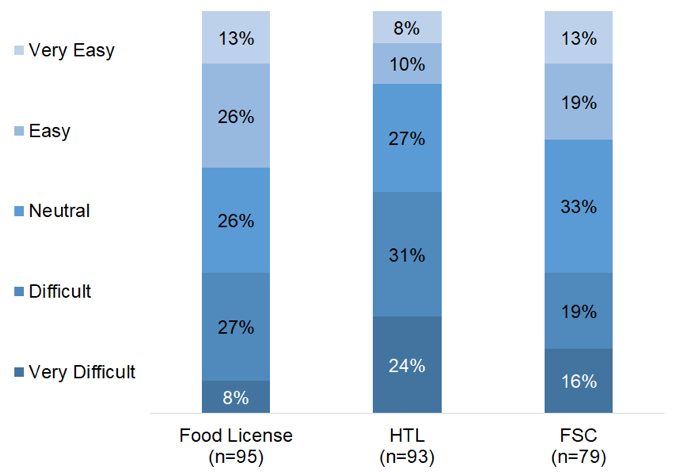
\includegraphics[height = 3.5in]{Figure1.png}
                    	\caption[Optional Caption]{Ease of Obtaining a Licence from the Food Safety and Standards Authority of India, South Delhi Municipal Corporation and Delhi Fire Services}
		\end{figure}
                
                   \subsubsection{Consent to Establish/Consent to Operate}
                   In September 2017, 21 restaurants were sealed in Hauz Khas Village, an urban village in South Delhi, for not having the necessary environment clearances—Consent to Establish (CTE) or Consent to Operate (CTO)—issued by the Delhi Pollution 
Control Committee (DPCC) (Hindustan Times 2017). Although the magistrate argued that the establishments were served ‘closure notices about 4 months ago’, the owners denied being served the notices (ibid). On the contrary, one of the restaurant owners 
claimed that he had applied for the DPCC certificate, but his application was put ‘on hold unnecessarily’ (ibid).\footnote{The confusion about the status of obtaining licences and closure notices, and the consequent sealing, affected not only restaurant owners but 
also the employees of the establishments. ‘Sealing these eateries has not only led to big losses for the owners but has affected the livelihood of 700 employees as well’ (Javaid, 25 Sept 2017).} Some restaurateurs claimed that the recent introduction of the 
digitisation process had created confusion among them about the renewal of licences, which delayed their usual procedure for getting their clearances renewed.% i dont understand the footnote in this. 
                   
                   Businesses such as eating houses that discharge sewage or effluents are required to obtain a CTE/CTO under Section 21 of the Air (Prevention and Control of Pollution) Act of 1981 and Section 25 of the Water (Prevention and Control of Pollution) Act 
of 1974.\footnote{\href{https://bit.ly/2pbaWOw}{The Air (Prevention and Control of Pollution) Act, 1981} (Accessed 31 June 2018).} \footnote{\href{https://bit.ly/2xcUyRW}{The Water (Prevention and Control of Pollution) Act, 1974} (Accessed 3 July 2018).}  %need to 
check if the hyperlink of the footnotes is correct. 
                   
                   Forty-two percent of survey respondents found the process for applying for the CTE/CTO either ‘difficult’ or ‘very difficult’. As against that, 23\% of respondents found it ‘easy’ or ‘very easy’ (Figure 2).
                          
                   \subsubsection{Shops and Establishment Certificate}
                   The Shops and Establishment Certificate (SEC) appears to be the easiest to obtain among all the others, with only 15\% (10 out of 65) respondents experiencing the process as ‘difficult’. It is issued by the Shops and Establishment Inspectorate within the Office of the Labour of Delhi under the Delhi Shops and Establishment Act 1954. The Act guarantees basic rights for employees, namely, working conditions, number of working hours in a week, holidays that the workers are entitled to, rights of women workers, intervals for rest and meals among other important rights.
         
         
                   \subsubsection{Eating House Licence}
                   The Eating House Licence is one of the more challenging ones to obtain; 49\% of 85 respondents found the procedure for obtaining the licence either ‘difficult’ or ‘very difficult’ (Figure 2).
                   
                   The licence is issued by the Office of the Additional Commissioner (licensing unit of the Delhi Police), as mandated by Section 28 (subsection za) of the Delhi Police Act, 1978. This licence serves to verify all the aforementioned licences issued.\\
                   If the licence only requires the submission of other licences, why is it so difficult to obtain? One of the respondents said that the practice of bribery had come to be widely regarded as a legitimate way of acquiring this licence. Although the process has 
been made online, long queues wind in front of the Eating House desk of the Licensing Unit of Delhi Police. Another respondent said, ‘The licence is delivered at your doorstep if you know the right price to pay’.
                   
                   In a glaring instance of unreasoned regulation, the Delhi Police Act 1978 does not specify the purpose of this licence. When questioned, the Inspector Executive of Licensing Branch of Delhi Police explained: ‘Delhi Police is a law-abiding authority and 
needs to know what is happening inside an establishment. Delhi Police issues Eating House Licence after confirming that the establishment has all the other licences’.
                   
                   Other metropolitan cities like Mumbai and Ahmedabad have done away with the Eating House Licence to facilitate ease of doing business (The Times of India 2018).\footnote{\href{https://bit.ly/2xiMwpL}{Circular No. BDD/384} issued by the Municipal 
Corporation of Greater Mumbai (dated 7 November 2016).} \footnote{On 26 March 2018, the Gujarat State Assembly \href{https://bit.ly/2xktGyu}{passed} the Gujarat Police (Amendment) Act, 2018, which exempted restaurants and eateries from obtaining a licence 
from the police to start their unit.}
                   
 			\begin{figure}[H]
                    		\centering
                    		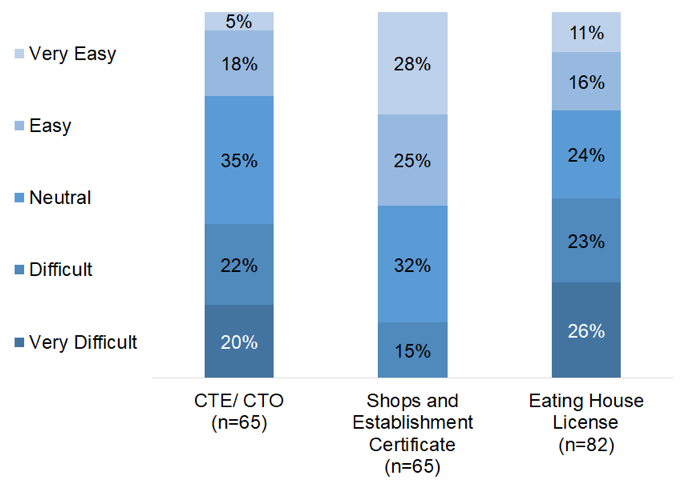
\includegraphics[height = 3.5in]{Figure2.png}
                    		\caption[Optional Caption]{Ease of Obtaining Licences from DPCC, Labour Department and Delhi Police}
			\end{figure}

		\subsubsection{Goods and Services Tax Registration}
		The latest addition to the list, registration for the GST became mandatory since 1 July 2017, when the GST Act came into force. Most respondents (78\% of 84) found the process of GST registration ‘easy’ or ‘very easy’ (Figure 3).
		
		\subsubsection{Signage Licence}\footnote{Placed under ‘Mandatory Licences’ because it is assumed that every restaurant and bar opts for a signage board.}
		Local Municipal Corporations issue the Signage Licence according to the Outdoor Advertising Policy 2017 of the Environment Pollution (Prevention and Control) Authority. A Signage Licence is required for the self-advertising boards that restaurants put 
up in front of their shops. A Signage Licence is needed to ensure that there are no instances of traffic hazards, obstacles to pedestrians, visual pollution or negative advertisements.\footnote{\href{https://bit.ly/2xdiNzk}{Delhi Outdoor Advertisement Policy 2008.}}
		
		\begin{figure}[H]
                    	\centering
                    	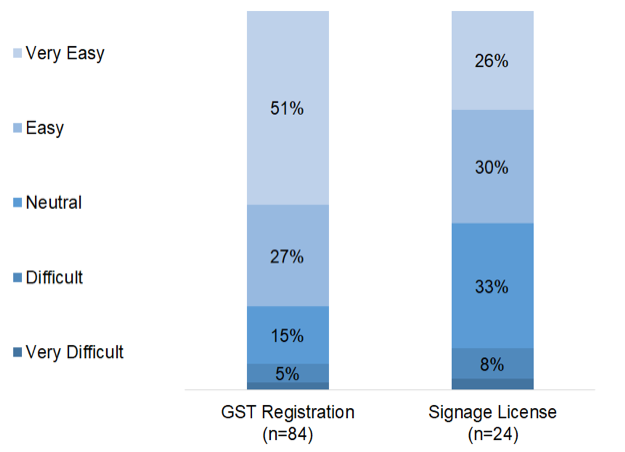
\includegraphics[height = 3.5in]{Figure3.png}
                    	\caption[Optional Caption]{Ease of Obtaining the GST Registration and Signage Licence from the South Delhi Municipal Corporation}
		\end{figure}
		
		\subsection{Service-specific Licences: Difficulties in Providing Value Addition}
		
		A restaurant may obtain five licences depending on its offering. These are required if a restaurant chooses to serve alcohol, play live music or install a lift in the establishment. The most expensive of these is an Excise Licence (required for serving liquor) 
with a mandatory increase of 10\% in the licence fee each year.\footnote{\href{https://bit.ly/2xoejoG}{Notification No. F.12(4)/Fin(Rev-I)/15-16.dsVI/587} from the Office of Commissioner of Excise (dated 29 July 2015).}
		
%Table 4: Time, Cost, Validity and Procedure of Service-Specific Licences in Delhi
%this is listed as table 4 in the word doc but really it is table 3. should we be deducting points from the proofer for missing this?
		\begin{table}
		\raggedright
		\caption{Time, Cost, Validity and Procedure of Service-Specific Licences in Delhi}
		\begin{tabular}{l | l | l | l | l | l | l)
			\bf{\thead{\footnotesize{Services}} & \bf{\thead{\footnotesize{Licences}} & \bf{\thead{\footnotesize{Days to Obtain}}} & \bf{\thead{\footnotesize{Official Cost \\(Rs.)}} & \bf{\thead{\footnotesize{Validity (Years)}} & \bf{\thead{\footnotesize{How to Apply}} & \bf{\thead{\footnotesize{Issuing Government}}\\
			\hline
			\multirow {3}{*}{Serving Alcohol} &	\multirow {2}{*}{Approval from the Department of Tourism} &	21	&	10,000 (up to 100 seats)		&5  &	Online		&	State\\
			&&&{15,000 (100+ seats)&&\\
		\end{tabular}
		\end{table}  		
		
		
		
		
	%================================================================
		
		\subsubsection{Approval from the Department of Tourism}
		An approval from the Department of Tourism (DoT) is a prerequisite to obtaining a licence from the Department of Excise to sell liquor.
		
		As mentioned on the website of DoT, this approval is given only to restaurants with a minimum seating capacity of 30.\footnote{\href{https://bit.ly/2NMdccI}{Terms and Conditions for Restaurants} as listed on the website of DoT.}  Since approval from the 
DoT is necessary to obtain an Excise Licence, the procedure to obtain the latter for restaurants with less than 30 seats is unclear. %this para was highlighted in the paper. i don't know how to do this, or if we should.
		
		
		\subsubsection{Excise Licence}
		The Excise Licence was rated as the most difficult to obtain among the 13 licences we sought feedback on. Of the 41 respondents, 59\% rated it ‘difficult’ or ‘very difficult’ (Figure 4). Restaurants that serve liquor need to obtain the L-17/L-17F/L-18/L-18F 
licences, issued under Section 20 of the Delhi Excise Act, 2009, by the Department of Excise, Government of Delhi.\footnote{L-17 is required to serve Indian liquor; L-17F is required to serve foreign liquor; L-18 is required to serve Indian wine, beer and alcopop; 
L-18F is required to serve foreign wine, beer and alcopop.} %removed the spaces b/w l17 and f
		
		In October 2016, the Government of Delhi directed the Department of Excise to not grant any new liquor licences to restaurants or retail vendors, as it believed that ‘the existing number of liquor vendors is enough to meet the demand of the city’ (Pandit 
2016). There was a strong backlash against the move. The National Restaurant Association of India (NRAI) raised two concerns:
		\begin {enumerate}
			\item Some restaurateurs had already invested in setting up their bars and paid the stipulated fee for acquiring the licence. The stalling resulted in a loss of business for these bar owners.
			\item Not granting licences to restaurants that provide ‘safe and licensed premises for liquor service’ would aggravate the law and order situation, as more people would drink at retail vends, in cars or on the roads (ibid).
		\end {enumerate}
		
		The ban lasted for 7 months. It was revoked in June 2017 because the government was convinced that ‘barring restaurants from serving liquor would serve no purpose, as people would drink at other places and cause problems’ (Kaushika 2017).
		
		The Excise Licence is the most expensive of all licences with a mandatory increase of 10\% in the licence fee each year.\footnote{\href{https://bit.ly/2xoejoG}{Notification No. F.12(4)/Fin(Rev-I)/15-16.dsVI/587} from the Office of Commissioner of Excise 
(dated 29 July 2015).} 
		
		
		\subsubsection{Weights and Measures Licence}
		The Controller of Weights and Measures issues this licence according to the Legal Metrology Act 2009. Every manufacturer, /dealer or /repairer of weights and measures is required to obtain this licence to carry out his/her trade. The purpose of the 
licence is to ensure that the customer is being served the right quantity of food or drink that he/she has ordered without being defrauded in any manner, either in quantity served or in price charged.
		
		Of 45 respondents, 61\% labelled it either ‘very easy’ or ‘easy’ to obtain (Figure 4). %why is the number of respondents on this only 45?
		
		Restaurateurs allege that inspecting officials extort money by wrongfully accusing the restaurant of serving an inadequate quantity of liquor. Officials are said to ask for a peg of whiskey, for instance, and pour it in a different beaker with etched 
measurements. The inspector then alleges fraud over the slight difference in measurement observed (owing to the residual drops naturally left in the first container). This compels restaurateurs to cough up bribes to keep their certificates or licence.
		
		\begin{figure}[H]
                    	\centering
                    	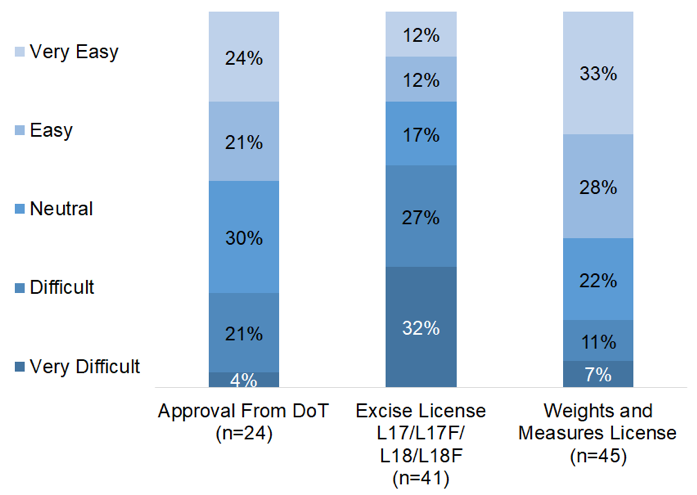
\includegraphics[height = 3.5in]{Figure4.png}
                    	\caption[Optional Caption]{Ease of Obtaining Approvals to Sell and Serve Alcohol}
		\end{figure}
	%i would like to change the bars to 'excise licenses' and remove the L-17 etc. neater. 
	
		\subsubsection{Lift Clearance}
		The Lift Inspectorate of the Office of the Labour Commissioner of Delhi is responsible for issuing the lift clearance. The Delhi Lift Rules of 1942 specify the standards for the installation of lifts, inspection of standards and the penalty to be paid in case of 
damage done to any user. The clearance is issued only after inspections have been conducted by officials of the Lift Inspectorate to ensure the safety of the installed lift. The lift has to satisfy standards set by the Bureau of Indian Standards.
		
		Forty percent of 30 respondents labelled it as either ‘very easy’ or ‘easy’ to obtain while only 7\% thought it was ‘difficult’ to obtain. %i don't understand why this is only 30 respondents. also shouldn't 'forty percent' be 40%
		
		
		\subsubsection{Phonographic Performance Licence}
		A music licence is necessary to play recorded music to protect the copyright of a music label or an artist. Phonographic Performance Limited, a non-governmental organisation, issues the music licence on behalf of the government, according to the 
Copyright Act of 1957. Of the 41 respondents, 46\% labelled the process as ‘easy’ or ‘very easy’ to obtain, whereas only 10\% thought it was ‘difficult’ or ‘very difficult’.
		
		In May 2018, the Department of Excise, Delhi, dispatched a circular to restobars that ‘only live singing/playing of instruments by professionals’ was allowed and that recorded music was banned.\footnote{\href{https://bit.ly/2MzCM02} {Order No. 2(72)/Ex/
Restt/Misc./2016-17/1567 (2018)} from the Office of Excise Commissioner, Delhi (dated 9 May 2018).} The blanket ban was to address the ‘nuisance caused by high volumes’, as most of the restobars are congregated near residential areas such as Hauz Khas 
Village and Khan Market (Jain 2018).
		
		The restaurateurs demanded a revision of the order, citing several reasons, such as recorded music is an essential part of the cultural experience of a restobar; the industry is heavily dependent on recorded music, as live music is expensive and cannot 
be played all day long; disallowing restobars from playing recorded music may not help reduce the ‘nuisance caused by high volumes’, as live music can be equally loud, if not louder; restaurants that don’t serve liquor do not come under the purview of excise rules 
but can be a cause of nuisance; and the problem could be better addressed by proper regulations such as volume control, which would suit everyone’s interests (ibid).
		
		\begin{figure}[H]
                    	\centering
                    	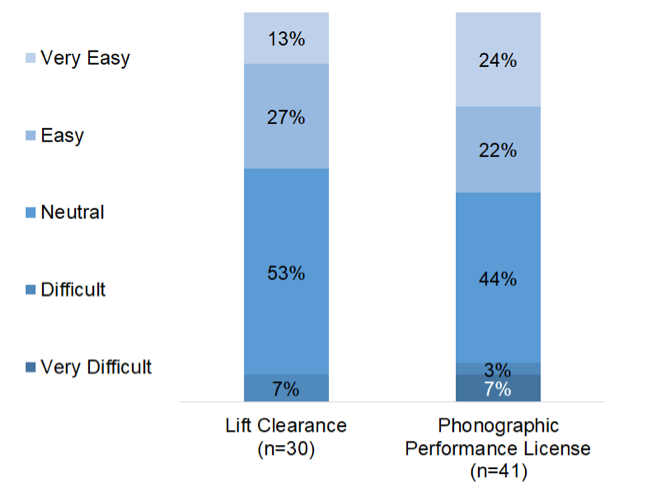
\includegraphics[height = 3.5in]{Figure5.png}
                    	\caption[Optional Caption]{Ease of Obtaining Lift Clearance from the Department of Labour, Phonographic Performance Limited}
		\end{figure}	
		
		\subsection{Overall Ease of the Licensing Procedure and Costs Involved}
		Fifty-six percent (51 out of 91) of the respondents found the overall licensing procedure difficult or very difficult to follow. Only 12\% (11 of 91) perceived the licensing procedure to be ‘easy’ or ‘very easy’, and the rest chose neutral. Out of 51 respondents 
who found the process difficult, 49 respondents revealed how they obtained the licences, 46.9\% applied for the licences by themselves, 22.4\% respondents applied through a third party and 10.2\% respondents had a specialised licensing team. It suggests that 
those who apply by themselves are more likely to find the process difficult.
		
		Fifty-three out of 93 respondents (57\%) paid a bribe to acquire licences. The number is an underestimate, as it is likely that many respondents felt uncomfortable while answering the question. For instance, some respondents verbally admitted to having 
paid a bribe but marked ‘No’ in the questionnaire.
		
		Interestingly, some restaurateurs did not fault the system and claimed that they paid bribes of their own volition to obtain the licence sooner. Others felt cornered into paying bribes. When officials raise repeated objections to the documents submitted, 
many feel that paying a bribe is the only option to obtain a licence in time.
		%this entire subsection was in the shaded box. not sure how to do it or if we should. 
		
		

%============================ENFORCEMENT OF THE REGULATORY FRAMEWORK=====================
	
		\section{Enforcement of the Regulatory Framework}
		\label{sec:2}
		
		Inspection is the primary mechanism to monitor compliance. For the Indian Food Services sector, inspections aim at ensuring food safety, fire safety, health and hygiene compliance and environment safety. In lieu of a single regulatory authority 
monitoring compliance across functions, multiple departments have their own brigade of inspectors. Thus, inspections are carried out independently and have different policies governing their nature, scope and due process.
		
		The restaurant industry of Delhi has been a constant target of compliance crackdown, resulting in frequent sealing drives in upscale areas such as Hauz Khas, Khan Market, Defence Colony and Connaught Place. In February 2017, the NDMC shut down 
21 rooftop restobars in Connaught Place in response to a partial collapse of a building in the market, citing the 'misuse of premises beyond sanction' under/Sections 250 and 252 of the NDMC Act, 1994 (The Times of India 2017). These restaurants were 
operational for decades, without permission, until the event of the collapse. It triggered a knee-jerk response from other regulatory bodies, resulting in large-scale closures.
		
		In another instance of compliance crackdown, a recent round of sealings of restaurants have been conducted in the aftermath of the Kamala Mills tragedy in Khan Market for flouting fire safety rules and illegal constructions (Firstpost 2018). This 
inconsistency in monitoring compliance creates uncertainty among businesses.
		
		\subsection{Restaurateur’s Perception of the Inspections Regime}
		Using an objective digitised survey, we tried to capture the restaurateurs’ perception of the way inspections are conducted. We asked the restaurateurs nine questions to understand the inspection regime and have discussed the three most pertinent and 
significant questions below, that is, what are they expected to do when faults are found, the intent of the inspectors and their perception of the inspectors.
		
		\subsubsection {What Are You Expected To Do When Faults Are Found?}
		Fifty-three respondents, almost half of the total, said that they had to fix the issue before the next inspection. Fifteen of the 53 respondents said that along with fixing the issue, they also had to pay a challan. Twenty-three of the 53 (43\%) respondents 
marked the options of fixing the issue and paying a bribe together. It appears as if the restaurateurs are required to comply with the legal and extra-legal demands of the inspectors. The restaurateurs appear to have to fulfil multiple expectations of fixing the issue, 
paying a formal challan and a bribe, simultaneously.

		\begin{figure}[H]
                    	\centering
                    	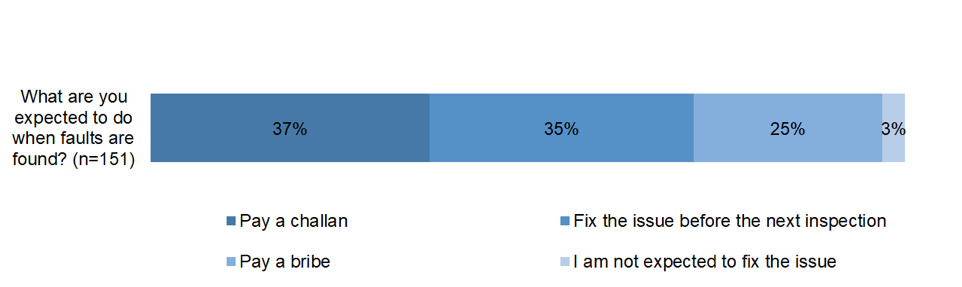
\includegraphics[width = 6.5in]{Figure6.png}
                    	\caption[Optional Caption]{Responses of Restaurateurs on What They Are Expected To Do When Faults Are Found by Inspecting Officials in Their Restaurants}
		\end{figure}

		
		\subsubsection {What Do You Think Is the Intent of the Inspectors?}
			When asked to describe the intentions of the inspectors, most respondents marked a combination of ‘To deliberately look for faults’ and ‘To further their personal benefit’. 28\% of the respondents thought that the inspectors visited with the intent of 
deliberately looking for faults. Thirty percent of the respondents felt that the intent of the inspectors when visiting restaurants is to further their own benefits.
		
		The choice for restaurateurs is often between paying a hefty challan and paying a lower amount as a bribe to the inspector in question. The existence of this system of bribery is borne out by the fact that 56\% of 100 respondents claimed to have paid a 
bribe in the course of inspections. Bribes are also collected in kind. Officers on duty often eat food in the restaurant they are inspecting and leave without paying the bill. Moreover, according to the responses of the restaurateurs we surveyed, officials bring their 
families to eat in the restaurant while off-duty and leave without paying the bill.
		
		Only a very small percentage of the people believed that the inspectors intended to either facilitate the ease of doing business for the restaurants or ensure the welfare of the customers.

		\begin{figure}[H]
                    	\centering
                    	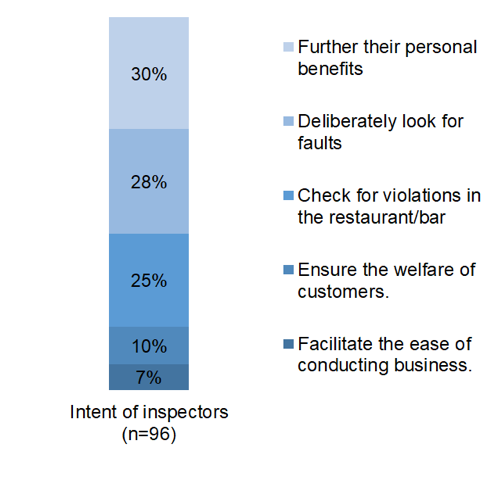
\includegraphics[height = 3.5in]{Figure7.png}
                    	\caption[Optional Caption]{Perception of Restaurateurs on the Intention of the Inspectors} %removed paying bribes from here. also need to try and redo this one so each option fits on one line
		\end{figure}

		\subsubsection {What Is Your Opinion of the Inspectors?}
				
		Inspections should be conducted in a transparent manner and in adherence to an ethical code of conduct (CIGIE 2012, p. 19). Inspectors ought to strive for a transparent communication system with the establishments to ensure compliance as far as 
possible. The inspectorates ought to perform the functions of information dissemination by drafting the regulations in a user-friendly manner and ensuring that establishments understand them (Jacobs and Cordova 2005).
		
		Survey respondents were asked to mark their level of agreement with four statements about inspectors. It is noteworthy that the two statements with which the majority of the respondents agree or strongly agree with are: ‘Inspectors treat you respectfully’ 
and ‘Inspectors are professional’. A caveat added by those who agreed with these statements was that the inspectors had to be respectful to them, as they had to ask for a bribe from them. It is also telling that the restaurateurs mostly admitted to paying a bribe at 
various stages of obtaining licences and inspections and still considered the conduct of the officials professional.
		
		\begin{figure}[H]
                    	\centering
                    	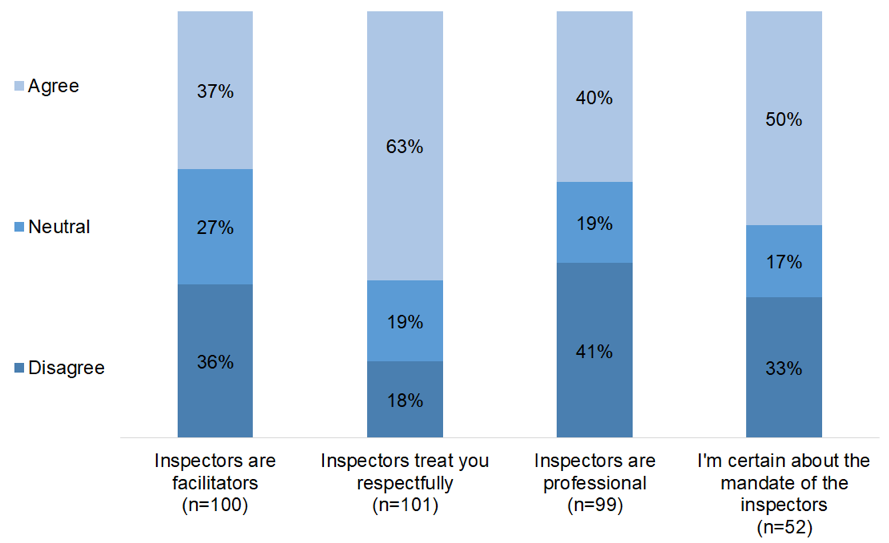
\includegraphics[height = 3.5in]{Figure8.png}
                    	\caption[Optional Caption]{Opinion of Restaurateurs About Inspectors} 
		\end{figure}


%======================OFT-REPEATED REGULATORY PAIN POINTS====================================

		\section{Oft-Repeated Regulatory Pain Points}
		\label{sec:3}
		
		In this section, we highlight and analyse some of the key pain points that eating houses repeatedly claimed to encounter while setting up and running a restaurant.
		
		\subsection{Efficiency of Web Portals}
		The Government of India is increasingly tapping into e-governance initiatives to enable the effective and efficient delivery of public services. The success or failure of e-governance initiatives hinges on the comfort with which customers can use the 
interface. Kinks in the website increase customer dissatisfaction with the portal and reduce the probability of their returning to it or recommending it to others (Anthopoulos, Siozos and Tsoukalas 2007, p. 10). 
		
		In our interaction with the restaurateurs, several respondents raised concerns about government websites, calling for a regular evaluation of their usability and credibility. For instance, during the course of our field research (June to July 2018), the 
website for registration under the Shops and Establishment Act applicable to all establishments within Delhi, including eating houses, was not functional.\footnote{\href{https://bit.ly/2xfB6UJ}{Registration form for Shops and Establishments} (Accessed 19 July 
2018).} Since the application for the Shops and Establishment licence can only be made online, in the absence of any alternatives, the inoperability of the website may have deprived the businesses set up during this period from the facility to apply for the licence. 
Besides this, two respondents also pointed out that the websites of the Department of Excise and the MCD were temporarily inoperative in the past. When government websites that facilitate functions such as licence application are non-functional without any 
intimation to businesses, it impedes the uptake of e-governance.
		
		Some of the application procedures are entirely online, some offline and for others, they are a combination. This leads to two problems: first, it increases the uncertainty faced by applicants, and second, procedures that are online only may not be 
accessible for the digitally illiterate. Digital literacy is almost non-existent for over 90\% of the population.\footnote{\href{https://bit.ly/2NMWdaj}{Digital Empowerment Foundation}}  Ambiguity around procedures creates scope for corruption and increases the cost of 
doing business. Partially online systems, such as with the Eating House Licence, require the restaurateurs to visit department offices to submit documents, collect them and make a payment, defeating the purpose of introducing a system meant to reduce the scope 
of human contact.
		
		\subsection{Pressure to Pay Bribes}
		Corruption, that is, an ‘an illegal payment to a public agent to obtain a benefit for a private individual or firm’, (Rose-Ackerman 1999, p. 373) is commonly accepted as a component of the application and inspection procedure. It is also difficult to measure, 
as the people involved are unlikely to accept complicity. Respondents pointed out that bribes are never asked for directly. According to one restaurateur, ‘The inspectors levy an exorbitant fine for a violation and then offer an \textit{easier way} out by asking for 
personal payment of a lower amount and waiving the fine’(emphasis added). This arrangement benefits both the restaurant and official.\\
		Although the government has attempted several measures, such as shifting the application process online, the absence of clear information and continuing discretionary powers continue to fuel the practice of grease payments. Restaurants complained, 
for example, that the Delhi Police Inspectors visit the restaurants intentionally at peak hours, creating anxiety and panic among the customers. Restaurateurs offer illegal payments just to ensure that the inspectors leave the establishment as soon as possible. This 
appears to be another systematised manner of seeking bribes.
				
		\subsection {Lack of Procedural Clarity}
		In 2017, unlicensed restaurants accounted for 66\% of the market share of the restaurant industry in India (Dabas 2017). Various reasons why firms choose to stay unregistered include for some, a want of access to finance, and for others, an avoidance 
of paying taxes. Some others do not register due to procedural difficulties. Although our respondents were only registered restaurants, 13 out of 43 respondents highlighted the lack of clear guidelines as a pain point. Restaurants seek a single point of reference for 
all necessary information necessary to be compliant. They are not informed of the new guidelines or directions in a structured manner. Even to compile details on the process of registration, we had to visit several websites and government offices.
		
		A defined way of intimating enterprises about new information or changes in regulations is not available. For example, the blanket ban on playing recorded music in restobars, imposed by the Department of Excise in May 2018, created much confusion 
for the restaurateurs. The order was allegedly passed following complaints from residents in the neighbourhood. Following protests from restaurateurs, the Deputy Chief Minister of Delhi, Manish Sisodia (The Hindu 2018) made a statement proposing to strike down 
the ban. However, the revised order published subsequently by the Department of Excise simply reiterated its previous order by stating ‘However in the case of L-17 licensee only live singing/playing of instruments by professionals shall be allowed’.
\footnote{\href{https://bit.ly/2QxMK56}{Order No. 2(72)/Ex/Restt/Misc./2016-17/1615 (2018)} from the Office of Excise Commissioner, Delhi (dated 22 May 2018).}  While the public concurrence of the Department with the Deputy Chief Minister leads one to believe 
that there is no such ban, a closer reading of the revised circular simply reveals that the rules remain unchanged. The lack of a clear stand publicly and in writing creates confusion in the minds of the restaurateurs.
		
		Another example of arbitrary policy changes and rule revisions is the decision to temporarily halt the issue of new Excise Licences in 2016 (Pandit 2016). One of our respondents lamented that he had invested in setting up a restobar and complied with 
all requirements but given the sudden policy change, had instead borne substantial losses. The lack of precise information is also why restaurateurs seek third-party ‘consultants’, increasing the cost that restaurateurs incur to set up their businesses. These 
consultants are generally either law firms that charge an exorbitant fee for their legal services or \textit{Dalals} who stand in front of government offices.\footnote{Dalals refer to the agents or facilitators stationed outside government offices and buildings, who help 
expedite paperwork in return for a fee.} Both these entities provide their services in return for a fee that serves as their income. A portion of that fee is also used to grease the hands of the relevant officials. Thus, bribery continues but is more targeted and precise.
		
		The erratic sealing drives on a variety of issues such as the use of terraces, the serving of hookah, the use of basements, etc. increase the uncertainty that restaurant businesses face. While many respondents understood that specific measures had to 
be taken for the safety of the customers, what they could not understand was why their restaurants had been permitted to function for so long and why closure was the proposed solution instead of grandfathered remediation, liability insurance and damage 
payments.


%================================CONCLUSION======================================

		\section*{Conclusion}
		\label{end}
		\addcontentsline{toc}{section}{Conclusion}
		
		The restaurant industry within the hospitality sector is a significant economic force. While the industry faces several obstacles to its growth, one of the pressing challenges restaurants face is the inconsistent and ever-changing regulatory framework. The 
NRAI, in 2016, commenting on the small proportion of licensed restaurants, said, ‘This is largely due to over-regulation of our industry, the complex maze of approvals and licences required and high tax brackets. It is about time that the socio-economic impact of 
our industry is recognised by the government, and it initiates immediate steps to unlock the true potential of this behemoth’ (NRAI 2016a).
		
		In this paper, we have systematically documented facts and perceptions around the regulatory framework governing eating houses in Delhi.
		
		A restaurant owner in Delhi requires a minimum of 8 and a maximum of 13 licences from 3 levels of government before he or she can open doors. This excludes the multiple NOCs required such as from the Delhi Jal Board, the Delhi Metro Rail 
Corporation and the Archaeological Survey of India among others. Besides these, the application requires to furnish over 50 documents, some of which are submitted more than once due to the involvement of multiple departments and a lack of inter-departmental 
coordination (Appendix 1). The time taken to obtain the licences and the addition to costs due to bribes probably explain why 56\% of the respondents in our study found the licensing procedure to be difficult or very difficult.%should we hyperref appendix 1?
		
		Respondents frequently raised concerns over the digitisation of the licensing procedure, as the websites are either poorly designed or often non-functional. Unfortunately, partially online processes continue to provide scope for corruption, as it does not 
eliminate human contact or the associated discretionary powers. Although the government has moved some of the processes entirely online, it excludes a sizeable digitally illiterate population from obtaining the necessary licences.
		
		Respondents also raised concerns about arbitrary and capricious rule changes, such as the ‘blanket ban on playing recorded music’ or the temporary ban on issuing new Excise Licences. Such changes, in the absence of reasoned orders that account for 
the impact on enterprises, increase the regulatory uncertainty faced by enterprises.
		
		We have not examined solutions to current regulatory challenges in this paper. However, a commonly proposed solution is to introduce a single-window system or a systematic reduction in the number of licences, to bring regulatory hygiene. Mumbai, for 
instance, implemented a single-window system for restaurants in 2017 with an upper limit of 27 days for completing the entire permit procedure. It intends to remove the overlap between licences and weed out irrelevant licences. In the case of Mumbai, ‘the number 
of general, special conditions and NOC required for such businesses’ have come down ‘from 72 to 51’ (NRAI 2016b).
		
		One of the licences done away with, in both Mumbai and Ahmedabad, is the Eating House Licence which is currently still issued by the Delhi Police. Since this licence is only a check on whether a restaurateur possesses all the other, essential licences, it 
cannot be said to be performing an important regulatory function.
		
		Another licence whose purpose needs to be reconsidered is the approval from the DoT. It appears to be an unnecessary prerequisite to apply for the Excise Licence. Indeed, it proves to be cumbersome for restaurateurs, considering the difference in the 
eligibility criterion of seating capacity, between the DoT and the Department of Excise.
		
		Another way to reduce the number of licences needed to open a restaurant is by potentially combining the functions of the DFS and the Lift Inspectorate, as both departments conduct a thorough investigation of the building plan before issuing the 
respective licences.
		
		We can reduce the regulatory burden on the restaurant industry without compromising on the quality of safety that is ensured for the customers using the various avenues and methods available.


                 
%===================================BIBLIOGRAPHY=================================================              
                          
% Print Bibliography

% \printbibliography[title={Bibliography}]
	
	
	
%=======================================APPENDIX=================================================              
	      
        
        %==================Appendix1
		\newpage      
		\section*{Appendix 1: Documents Required for Licences\footnote{Excluding the GST, Signage, Weights and Measures, Lift Clearance and Phonographic Performance Limited.}}
		\label {Appendix1}
		\addcontentsline{toc}{section}{Appendix 1: Documents Required for Licences}
         
		\begin{figure}[H]
                    	\centering
                    	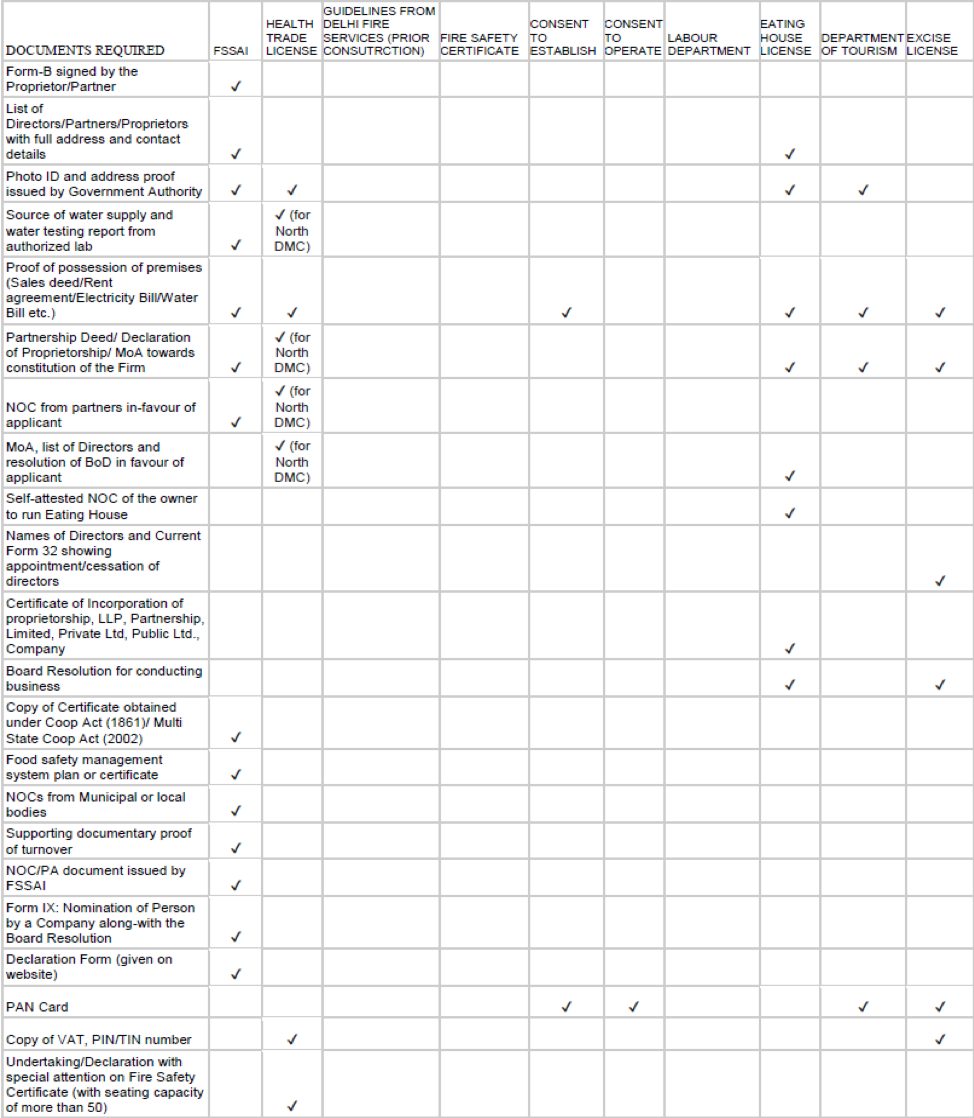
\includegraphics{Appendix1 - pg1.png} 
		\end{figure}

		\begin{figure}[H]
                    	\centering
                    	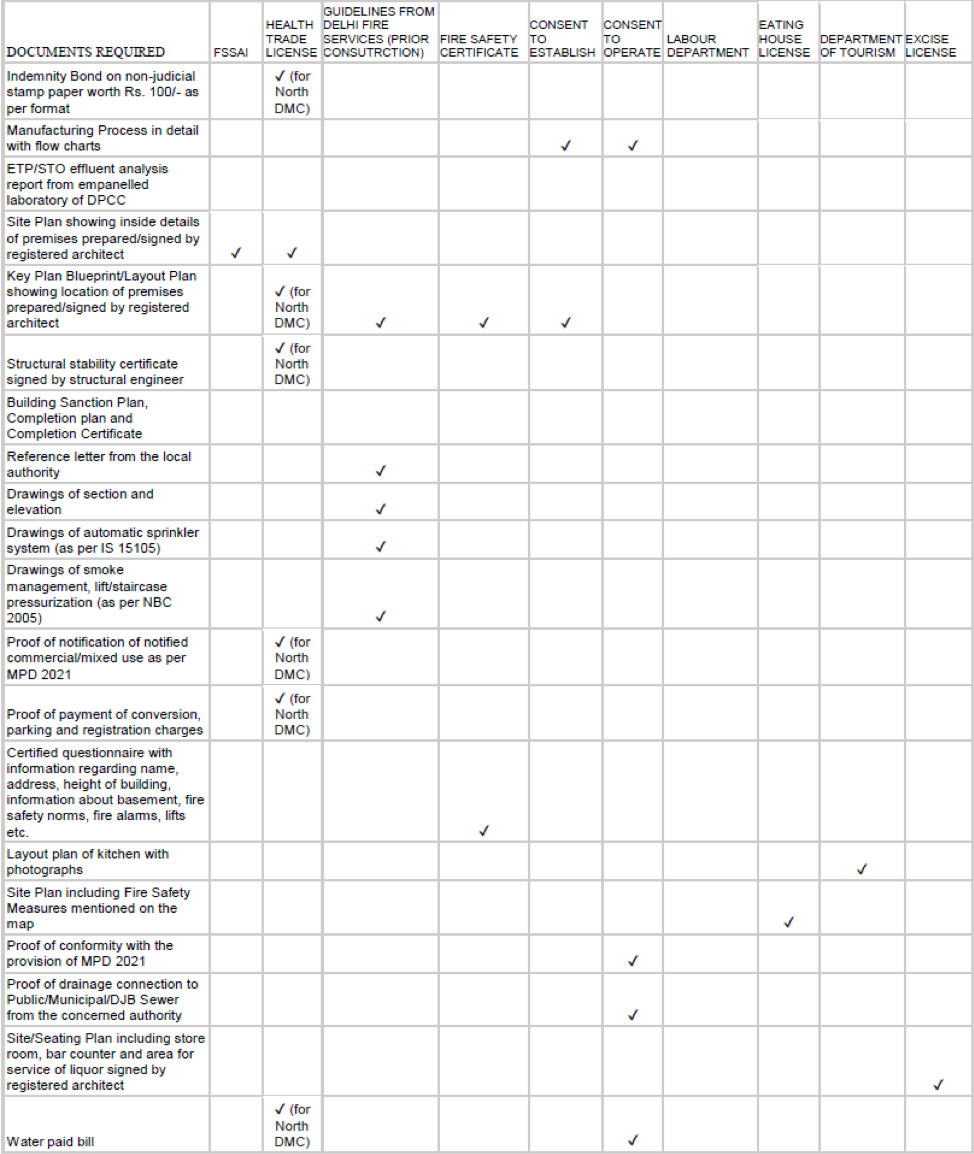
\includegraphics{Appendix1 - pg2.png} 
		\end{figure}
		
		\begin{figure}[H]
                    	\centering
                    	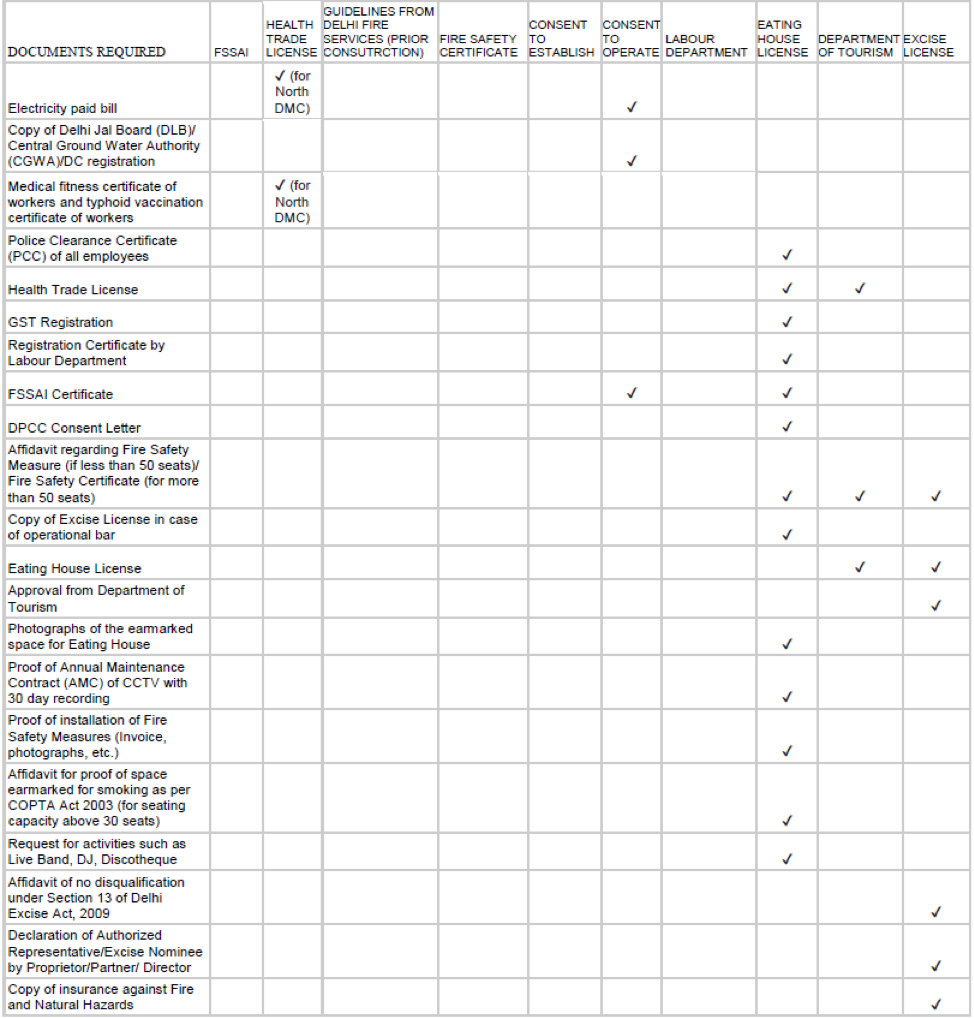
\includegraphics{Appendix1 - pg3.png} 
		\end{figure}
        
        %not sure why it is showing '- pg3.png' on top of each of the three pages
        
        
        %==================Appendix2
		\newpage
		\section*{Appendix 2: Methodology}
		\label {Appendix2}
		\addcontentsline{toc}{section}{Appendix 2: Methodology} 
		To understand the licensing and inspection procedure for restaurants and bars in Delhi, we relied on a survey of restaurateurs supported by semi-structured interviews with government officials. We also examined digitally available Acts, circulars, rules 
and procedures and orders as part of our exploratory research.
		
		\subsection* {Restaurant Survey}
		\textit{Sample}: We surveyed 101 food service enterprises in the central and south zones of South Delhi Municipal Corporation (SDMC), as the area features many markets and restaurant clusters. The survey was primarily administered to the owners. In 
case they were not available, we interviewed managers or members of the licensing department.

		\begin{table}[htpb]
			\raggedright
			\caption{Areas Covered Under SDMC}
			\begin{tabular}{ l  c  c | l  c  c}
			\bf{\thead{\normalsize{Area}} & \bf{\thead{\normalsize{Zone}} & \bf{\thead{\normalsize{Responses}} & \bf{\thead{\normalsize{Area}} & \bf{\thead{\normalsize{Zone}} & \bf{\thead{\normalsize{Responses}} \\
			\hline
				Adchini 			&	South		&	3				&	RK Puram			&	South	&	3	\\
				Chhattarpur		&	South		&	5				&	Safdarjung Enclave	&	South	&	3	\\
				Greater Kailash 1	&	South		&	5				&	Saket			&	South	&	3	\\
				Green Park		&	South		&	5				&	Satya Niketan		&	South	&	11	\\
				Hauz Khas Market	&	South		&	6				&	SDA Market		&	South	&	6	\\
				Hauz Khas Village	&	South		&	7				&	Amar Colony		&	Central	&	3	\\
				Humayunpur		&	South		&	4				&	Defence Colony	&	Central	&	3	\\
				Kailash Colony		&	South		&	5				&	Greater Kailash 2	&	Central	&	7	\\
				Katwaria Sarai		&	South		&	2				&	Lajpat Nagar 2		&	Central	&	2	\\
				Malviya Nagar		&	South		&	7				&	New Friends Colony	&	Central	&	7	\\
				Mehrauli			&	South		&	4							
			\end{tabular}
		\end{table}    
   		
		%SO UGLY. Need to fix. 
		
		
		We sought to survey restaurants along four parameters:
		\begin{enumerate}[nosep]
			\item Does the restaurant serve non-vegetarian food?
			\item Does the restaurant sell liquor?
			\item Is the restaurant located in an urban village?\footnote{From time to time, rural settlements are shifted into the urban ambit and are declared as ‘urban villages’. A notification is issued under Clause (a) of Section 507 of The Delhi Municipal 
Corporation Act, 1957. At present, there are 135 urban villages in Delhi. Norms for these villages are laid down in the Master Plan Delhi 2021, however, these villages remain exempted from sealing.} 
			\item Is the restaurant part of a chain? \footnote{According to Federation of Indian Chambers of Commerce and Industry, restaurants with three or more outlets are a part of chains.}
		\end{enumerate}

		\begin{figure}[H]
                    	\centering
                    	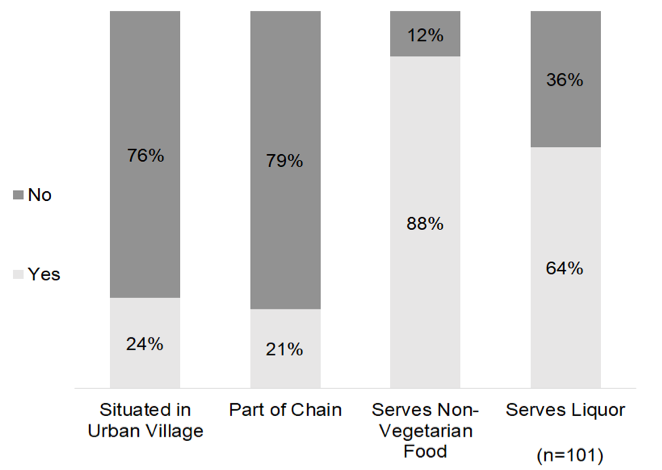
\includegraphics[height = 3in]{Figure9.png}
                    	\caption[Optional Caption]{Parameters for the Sample}%edited the caption 
		\end{figure}

		\textit{Survey Questionnaire}: The questionnaire (Appendix 3) consisted of five sections. First, we collected basic information on the respondent and the eating house. Second, we focused on the ease or difficulty in the process of obtaining licences and 
approvals.\footnote{Questions on ease of obtaining approval from the DoT were added mid-way during our survey, as we only found out the need for these two during the course of administering the survey to restaurateurs.} The third section had questions on 
experience with the licence renewal process. Fourth, we captured the experience of owners, managers and staff with inspections. The last section consists of questions to capture the perception restaurateurs held of the inspecting officials.

		\subsection*{Semi-Structured Interviews with Government Officials}
		We interviewed officers, inspectors and executives of various government departments to understand the purpose, procedure and motivation behind the different practices and licences. We interviewed officials of various departments about the purpose, 
application process, fee, eligibility, validity, renewal process and renewal fee of the licences and approvals under their ambit. We also asked them questions pertaining to the inspection procedure: frequency of inspections, number of inspectors, mandate of 
inspectors, inspection checklists, inspection reports and if there was a grievance redressal system in case the restaurateur feels dissatisfied with the inspection process.
		
		Specific questions for certain departments included the following:\\
		\paragraph \textit {Department of Excise}
			\begin {enumerate}[nosep]
			\item How long does it take you to approve one purchase order? 
			\item What is the rationale behind banning recorded music in these restaurants?
			\item Restaurants are live streaming music. How does it solve the problem the order hoped to resolve?
			\end {enumerate}
		\paragraph \textit {Department of Labour}
			\begin {enumerate}[nosep]
			\item Why is the website not working? 
			\item Can the workers approach the department in case of any problems faced?
			\item What is your relationship with the labour unions?
			\end {enumerate}
		\paragraph \textit {Delhi Fire Services}
		\begin {enumerate}[nosep]
		\item What is the average time within which the licence is received?
		\item Restaurants in Khan Market were asked to obtain their licences in 15 days. Was that feasible for the department?
		\end {enumerate}


       %==================Appendix 3  
		\newpage
		\section*{Appendix 3: Questionnaire for Restaurateurs}
		\label {Appendix3}
           	\addcontentsline{toc}{section}{Appendix 3: Questionnaire for Restaurateurs}
	
	\subsubsubsection {Section 1: Restaurant Information}
		\begin {enumerate}[nosep]
		\item Please state your name. (Optional)
		\item Please state your designation. (Owner, Manager, Other)
		\item What is your restaurant/bar name? (Optional)
		\item Does your restaurant serve liquor? (Y/N)
		\item Does your restaurant serve non-vegetarian food? (Y/N)
		\item Is your restaurant part of a chain or not? (Y/N)
		\item What is the seating capacity of your restaurant?
		\item Is your restaurant part of any association? If yes, which one?
		\item State the location, market area or landmark of your restaurant or bar.
		\end {enumerate}
		
	\subsubsubsection {Section 2: Ease of Obtaining Licenses}
		\begin {enumerate}[nosep]
		\item How easy is it to obtain licences from the following department?\\ 
		\textit{Very Easy, Easy, Neutral, Difficult, Very Difficult}
			\begin {enumerate}[nosep]
			\item Food Safety and Standards Authority of India (FSSAI)
			\item Municipal Corporation (Health Trade Licence)
			\item Delhi Fire Services (Fire NOC/Fire Safety Certificate)
			\item Delhi Pollution Control Committee (CTO/CTE)
			\item Department of Excise (L17/L17F Licence)
			\item Department of Tourism
			\item Delhi Police (Eating House Licence)
			\item GST Registration
			\item Department of Labour (Shops and Establishment Licence)
			\item Employees State Insurance Provident Fund
			\item Department of Weights and Measures
			\item Department of Labour (Lift Clearance)
			\item Phonographic Performance Limited (Music Licence)
			\item Signage Licence
			\item Value-Added Tax Registration (For Liquor)
			\item Overall Licensing Procedure
			\end {enumerate}
		\item How long did it take you to obtain all the licences? (In Months)
		\item After the sanctioning of building plans, were you asked to make any structural changes over the course of inspections? (Y/N)
		\item When you were applying for licences, did you pay a bribe? (Y/N)
		\item What amount did you pay as a bribe? (Optional)
		\item How did you apply for the licences?\\
		\textit{Self, Consultants, Both, Licensing Team}
		\end {enumerate}

	\subsubsubsection {Section 3: Application and Renewal of Licenses}\\
		\begin {enumerate}[nosep]
		\item Are you aware of the online application process? Has it made the process easier?\\
		\textit{Yes, I find the process easy; Yes, I find the process difficult; No, I am not aware}
		\item How simple do you find the online renewal process?\\
		\textit{Very Easy, Easy, Neutral, Difficult, Very Difficult}
		\item How simple do you find the frequent renewal of licences?\\
		\textit{Very Easy, Easy, Neutral, Difficult, Very Difficult}
		\end {enumerate}

	\subsubsubsection {Section 4: Inspections process}
		\begin {enumerate} [nosep]
		\item What is the duration between two inspections?
		\item Which four authorities/departments come for inspections most frequently?
		\item Can you challenge the way any inspections are conducted or their findings? (Y/N)
		\end {enumerate} 

	\subsubsubsection {Section 5: Perception about Inspectors}
		\begin {enumerate}[nosep]
		\item What is your opinion about the inspectors? (Agree, Neutral, Disagree)
			\begin {enumerate}[nosep]
			\item Inspectors are facilitators
			\item Inspectors treat you respectfully
			\item Inspectors are professional
			\item I’m certain about the mandate of the inspectors
			\end {enumerate}
		\item What do you think is the intent of the inspectors? (You can select more than one.)
			\begin {enumerate}[nosep]
			\item To facilitate the ease of conducting your business
			\item To check for violations in the restaurant or bar
			\item To ensure the welfare of your customers
			\item To deliberately look for faults
			\item To further their personal benefits
			\end {enumerate}
		\item Are you aware of what is expected of you before inspections are carried out?(Y/N)
		\item My establishment faces overlapping regulations. (Agree, Neutral, Disagree)
		\item What are you expected to do when faults are found during inspections?\\
		\textit{Fix issue before next inspection; Pay challan; Pay bribe; Not expected to fix issue}
		\item Did you pay bribes during inspections post opening restaurant? (Y/N)
		\item Does the same inspector come for back-to-back inspections? (Y/N)
		\item What are the pain points you encountered in starting and running a restaurant?
		\item What reforms would you like to see being implemented with regard to regulatory compliances in the industry?
		\end {enumerate}
       

%reformatted the questionnaire from the word version. enumerate [a] doesnt work
                    
                    
 %================================Appendices over                   
                    
\end{document}

    		
  %====================== Code examples for table and figures====================================                 
                            
%table1         
\begin{table}[htpb]
\caption{Official Cost of Acquiring CTE and CTO}
\begin{tabular}{ l  c  c  c }
\thead{\normalsize{State}} & \thead{\normalsize{Licence}} & \thead{\normalsize{Cost in Rs.}\\ \scriptsize\textit{(For Investment Between 1 and 10 crores)}} & \thead{\normalsize{Official Time Taken}\\ \scriptsize\textit{(in days)}} \\
\hline
Uttar Pradesh & CTE + CTO & 1,17,000 & 40-60\\ 
Haryana & CTE + CTO & 3,84,000 & 20-40\\

\end{tabular}
\end{table}
                    
  %==============
